\documentclass[11pt,a4paper]{article}
\usepackage[margin=2.3cm]{geometry}
\usepackage{microtype}
\usepackage{setspace}
\usepackage{float}
\usepackage{caption}
\usepackage{hyperref}
\usepackage[table]{xcolor}
\makeatletter
\def\input@path{{.}{docs/}{./docs/}{../docs/}}
\makeatother
% shared notation and packages for slides.tex and report.tex
\usepackage{amsmath,amssymb}
\usepackage{booktabs}
\usepackage{graphicx}
\usepackage{siunitx}
\usepackage{xcolor}
\usepackage{tikz}
\usetikzlibrary{arrows.meta,positioning,shapes.geometric,calc}
\makeatletter
\providecommand{\input@path}{}
\g@addto@macro\input@path{{.}{docs/}{./docs/}{../docs/}}
\makeatother
\graphicspath{{../figures/}{figures/}{docs/figures/}}
% generated by code/12_export_tex.py -- do not edit by hand
\newcommand{\VfourMaize}{0.018}
\newcommand{\VfourPwMaize}{0.005}
\newcommand{\VfourPwRice}{0.001}
\newcommand{\VfourPwSoybean}{0.009}
\newcommand{\VfourPwWheat}{0.084}
\newcommand{\VfourRice}{0.002}
\newcommand{\VfourSoybean}{0.008}
\newcommand{\VfourWheat}{0.065}
\newcommand{\adqYears}{2021--2023}
\newcommand{\bTMaizeSAfrica}{-27.8}
\newcommand{\bTMaizeUSA}{-6.4}
\newcommand{\bTRiceIndia}{-11.4}
\newcommand{\bTWheatIndia}{-4.2}
\newcommand{\bWMaizeSAfrica}{+0.0}
\newcommand{\bWMaizeUSA}{+0.0}
\newcommand{\bWRiceIndia}{+0.0}
\newcommand{\bWWheatIndia}{+0.0}
\newcommand{\bdRiceKcal}{63}
\newcommand{\bdRiceZinc}{55}
\newcommand{\bdShockKcal}{-6.3}
\newcommand{\bdShockKcalAbs}{6.3}
\newcommand{\bdShockMar}{-0.50}
\newcommand{\egWheatIron}{46}
\newcommand{\egWheatKcal}{34}
\newcommand{\egWheatSone}{-3.6}
\newcommand{\egWheatZinc}{48}
\newcommand{\exEheat}{1.00}
\newcommand{\exEwater}{0.33}
\newcommand{\exI}{0.222}
\newcommand{\exImax}{0.421}
\newcommand{\exIn}{0.53}
\newcommand{\exLheat}{0.58}
\newcommand{\exLwater}{17.8}
\newcommand{\exSheat}{0.43}
\newcommand{\exShlit}{0.50}
\newcommand{\exShobs}{0.36}
\newcommand{\exSwater}{0.44}
\newcommand{\exSwlit}{0.88}
\newcommand{\exSwobs}{0.00}
\newcommand{\exVfour}{0.151}
\newcommand{\feRatioBangladesh}{0.70}
\newcommand{\feRatioBrazil}{0.97}
\newcommand{\feRatioEgypt}{1.20}
\newcommand{\feRatioIndia}{0.89}
\newcommand{\feRatioNigeria}{0.91}
\newcommand{\feRatioRussia}{1.14}
\newcommand{\feRatioSAfrica}{0.82}
\newcommand{\heatCellsMaize}{7}
\newcommand{\heatCellsRice}{2}
\newcommand{\heatCellsSoybean}{0}
\newcommand{\heatCellsWheat}{22}
\newcommand{\inRiceSone}{-4.8}
\newcommand{\inWheatKcal}{-2.1}
\newcommand{\inWheatMar}{-0.52}
\newcommand{\inWheatMarTrade}{-0.28}
\newcommand{\koppenAgree}{93}
\newcommand{\koppenAgreeMaize}{92}
\newcommand{\koppenAgreeRice}{93}
\newcommand{\koppenAgreeSoybean}{95}
\newcommand{\koppenAgreeWheat}{83}
\newcommand{\maizeFeedBrazil}{75}
\newcommand{\maizeFeedChina}{72}
\newcommand{\maizeFeedUS}{46}
\newcommand{\maizeFeedWorld}{60}
\newcommand{\maizeFoodSAfrica}{40}
\newcommand{\maizeFoodWorld}{12}
\newcommand{\marBangladesh}{0.939}
\newcommand{\marBrazil}{0.994}
\newcommand{\marEgypt}{1.000}
\newcommand{\marIndia}{0.978}
\newcommand{\marNigeria}{0.981}
\newcommand{\marRussia}{1.000}
\newcommand{\marSAfrica}{0.964}
\newcommand{\mcFourMaizeFirst}{1.0}
\newcommand{\mcFourRiceFirst}{0.0}
\newcommand{\mcFourSoybeanFirst}{1.5}
\newcommand{\mcFourWheatFirst}{97.5}
\newcommand{\mcOneMaizeFirst}{1.0}
\newcommand{\mcOneRiceFirst}{0.0}
\newcommand{\mcOneSoybeanFirst}{1.3}
\newcommand{\mcOneWheatFirst}{97.7}
\newcommand{\nCountriesAdq}{205}
\newcommand{\nPassNew}{26}
\newcommand{\nPassNewSig}{1}
\newcommand{\nPassOld}{26}
\newcommand{\nPassOldSig}{9}
\newcommand{\nRobustT}{7}
\newcommand{\nRobustW}{5}
\newcommand{\nShared}{5}
\newcommand{\nShock}{26}
\newcommand{\orderFour}{Wheat $>$ Maize $>$ Soybean $>$ Rice}
\newcommand{\orderFourPw}{Wheat $>$ Soybean $>$ Maize $>$ Rice}
\newcommand{\orderOne}{Wheat $>$ Maize $>$ Soybean $>$ Rice}
\newcommand{\pShock}{0.170}
\newcommand{\pShockE}{0.169}
\newcommand{\pShockS}{0.467}
\newcommand{\panelShareMaize}{69}
\newcommand{\panelShareRice}{63}
\newcommand{\panelShareSoybean}{90}
\newcommand{\panelShareWheat}{51}
\newcommand{\passRiceBangladesh}{0.37}
\newcommand{\passRiceChina}{0.90}
\newcommand{\passRiceIndia}{0.37}
\newcommand{\passSoyHi}{1.8}
\newcommand{\passSoyLo}{1.6}
\newcommand{\poolTMaize}{-11.7}
\newcommand{\poolTRice}{-1.1}
\newcommand{\poolTSoybean}{-6.2}
\newcommand{\poolTWheat}{-2.7}
\newcommand{\poolTpMaize}{0.000}
\newcommand{\poolTpRice}{0.476}
\newcommand{\poolTpSoybean}{0.000}
\newcommand{\poolTpWheat}{0.019}
\newcommand{\poolWMaize}{+1.5}
\newcommand{\poolWRice}{+0.3}
\newcommand{\poolWSoybean}{+1.8}
\newcommand{\poolWWheat}{-2.4}
\newcommand{\poolWpMaize}{0.079}
\newcommand{\poolWpRice}{0.422}
\newcommand{\poolWpSoybean}{0.020}
\newcommand{\poolWpWheat}{0.080}
\newcommand{\pshareIronMaize}{8.3}
\newcommand{\pshareIronRice}{9.4}
\newcommand{\pshareIronSoybean}{1.2}
\newcommand{\pshareIronWheat}{32.8}
\newcommand{\pshareProteinMaize}{5.1}
\newcommand{\pshareProteinRice}{13.4}
\newcommand{\pshareProteinSoybean}{0.6}
\newcommand{\pshareProteinWheat}{21.9}
\newcommand{\pshareZincMaize}{7.6}
\newcommand{\pshareZincRice}{15.3}
\newcommand{\pshareZincSoybean}{0.5}
\newcommand{\pshareZincWheat}{32.5}
\newcommand{\rankFourMaize}{2}
\newcommand{\rankFourPwMaize}{3}
\newcommand{\rankFourPwRice}{4}
\newcommand{\rankFourPwSoybean}{2}
\newcommand{\rankFourPwWheat}{1}
\newcommand{\rankFourRice}{4}
\newcommand{\rankFourSoybean}{3}
\newcommand{\rankFourWheat}{1}
\newcommand{\rhoShock}{+0.20}
\newcommand{\rhoShockE}{+0.19}
\newcommand{\rhoShockS}{+0.02}
\newcommand{\rhoZhaoClim}{+0.8}
\newcommand{\rhoZhaoFour}{+0.6}
\newcommand{\rhoZhaoFourPw}{+0.0}
\newcommand{\rhoZhaoHeat}{+0.8}
\newcommand{\rhoZhaoOne}{+0.6}
\newcommand{\rhoZhaoPool}{+0.4}
\newcommand{\riskIronMaize}{0.48}
\newcommand{\riskIronRice}{0.49}
\newcommand{\riskIronSoybean}{0.05}
\newcommand{\riskIronWheat}{1.67}
\newcommand{\riskProteinMaize}{0.00}
\newcommand{\riskProteinRice}{1.05}
\newcommand{\riskProteinSoybean}{0.00}
\newcommand{\riskProteinWheat}{1.38}
\newcommand{\riskZincMaize}{0.00}
\newcommand{\riskZincRice}{0.51}
\newcommand{\riskZincSoybean}{0.02}
\newcommand{\riskZincWheat}{3.02}
\newcommand{\robN}{80}
\newcommand{\robWheatTopAll}{80}
\newcommand{\rtwoMaize}{0.24}
\newcommand{\rtwoMaxMaize}{0.50}
\newcommand{\rtwoMaxRice}{0.26}
\newcommand{\rtwoMaxSoybean}{0.54}
\newcommand{\rtwoMaxWheat}{0.22}
\newcommand{\rtwoMinMaize}{0.05}
\newcommand{\rtwoMinRice}{0.01}
\newcommand{\rtwoMinSoybean}{0.05}
\newcommand{\rtwoMinWheat}{0.02}
\newcommand{\rtwoRice}{0.04}
\newcommand{\rtwoSoybean}{0.17}
\newcommand{\rtwoWheat}{0.13}
\newcommand{\saMaizeSone}{-26.8}
\newcommand{\sharedPanel}{Brazil, China, India, Russia, USA}
\newcommand{\sharedWheatTop}{5}
\newcommand{\skillMedian}{0.31}
\newcommand{\skillN}{21}
\newcommand{\skillPos}{18}
\newcommand{\snrHeatMaize}{0.68}
\newcommand{\snrHeatRice}{0.92}
\newcommand{\snrHeatSoybean}{0.64}
\newcommand{\snrHeatWheat}{0.80}
\newcommand{\soyFoodWorld}{4}
\newcommand{\soyProcChina}{81}
\newcommand{\soyProcUS}{92}
\newcommand{\soyProcWorld}{86}
\newcommand{\tauOneFour}{0.91}
\newcommand{\tauOneThree}{0.58}
\newcommand{\worldFatMaize}{1.4}
\newcommand{\worldFatRice}{1.8}
\newcommand{\worldFatSoybean}{12.5}
\newcommand{\worldFatWheat}{3.5}
\newcommand{\worldIMaize}{4.2}
\newcommand{\worldIRice}{10.2}
\newcommand{\worldISoybean}{4.5}
\newcommand{\worldIWheat}{18.7}
\newcommand{\worldIronMaize}{5.6}
\newcommand{\worldIronRice}{7.6}
\newcommand{\worldIronSoybean}{3.3}
\newcommand{\worldIronWheat}{26.0}
\newcommand{\worldKcalMaize}{4.9}
\newcommand{\worldKcalRice}{17.1}
\newcommand{\worldKcalSoybean}{3.7}
\newcommand{\worldKcalWheat}{17.8}
\newcommand{\worldProteinMaize}{3.3}
\newcommand{\worldProteinRice}{11.4}
\newcommand{\worldProteinSoybean}{1.8}
\newcommand{\worldProteinWheat}{18.8}
\newcommand{\worldZincMaize}{5.8}
\newcommand{\worldZincRice}{13.1}
\newcommand{\worldZincSoybean}{1.3}
\newcommand{\worldZincWheat}{27.2}
\newcommand{\worstMar}{-0.53}
\newcommand{\worstMarCase}{Maize in S. Africa}



\definecolor{rice}{HTML}{2A7F62}
\definecolor{wheat}{HTML}{C8961A}
\definecolor{maize}{HTML}{C0504D}
\definecolor{soy}{HTML}{5B5EA6}
\definecolor{ink}{HTML}{222222}
\definecolor{muted}{HTML}{6B6B6B}
\definecolor{paddy}{HTML}{1F4E3D}
\definecolor{grain}{HTML}{C8961A}
\definecolor{clay}{HTML}{B5523B}
\newcommand{\Teff}{T_{\mathrm{eff}}}
\newcommand{\Tcrit}{T_{\mathrm{crit}}}
\newcommand{\ETc}{\mathrm{ET_c}}
\newcommand{\ETo}{\mathrm{ET_0}}
\usepackage{adjustbox}


\usepackage[round]{natbib}
\usepackage{booktabs}
\bibliographystyle{plainnat}
\let\parencite\citep
\let\textcite\citet
\hypersetup{colorlinks=true,linkcolor=paddy,citecolor=paddy,urlcolor=paddy}
\captionsetup{font=small,labelfont=bf}
\setstretch{1.07}
\setlength{\parskip}{0.45em}
\setlength{\parindent}{0pt}
\newcommand{\TT}{\mathrm{T}}   % temperature
\newcommand{\PP}{\mathrm{P}}   % precipitation

\title{\textbf{Appendix to the Climate--Nutrition Vulnerability Study}\\[0.3em]
\large Detailed methodology, robustness tests, and supplementary tables for rice, wheat, maize and soybean}
\author{Arpit Mahtele \and Dev Patel \and Navey Puri \and Shreyash Lohare}
\date{Earth 616}

\begin{document}
\maketitle
\tableofcontents
\newpage

% =====================================================================
\section{Calculation methodology}\label{sec:calc}
\subsection{Where each ingredient comes from}
This table summarizes the literature basis and methodological role of each analytical component. The individual ingredients are grounded in peer-reviewed and international agency sources (FAO, WHO, IPCC), while the hazard-paired combination (F4) is our specific index design.

\begin{table}[H]\centering\footnotesize
\begin{tabular}{p{4.2cm}p{5.6cm}p{4.6cm}}
\toprule
Ingredient & Literature backing & Status / Role in project\\
\midrule
Heat limit $T_{crit}$, $T_{lim}$ \& flowering window (45--70\% of season) & \textcite{deryng2014}; rice: \textcite{yoshida1981}, \textcite{jagadish2007} & Published values\\
Water need $ET_c = K_c \times ET_0$; Hargreaves $ET_0$ & \textcite{fao56}, Eq.~52 & Published method\\
Water factor $K_y$ & \textcite{fao66}, Table~1; \textcite{brouwer1986} & Published values\\
Signal-to-noise shift & \textcite{hawkins2012} & Published idea (robustness check only)\\
Observed yield regressions & \textcite{lobell2007}; \textcite{ray2015} & Out-of-sample data check / validation\\
Literature sensitivity $S^{\TT}, S^{\PP}$ & \textcite{deryng2014}; \textcite{fao66} & Primary sensitivity scale\\
Importance $I = \tfrac15\sum(\text{share of 5 nutrients})$ & FAO FBS and USDA FoodData Central & Core index ingredient\\
Mean Adequacy Ratio (MAR) & \textcite{who2003}, \textcite{whofao2004} requirements; \textcite{torheim2004} & Published adequacy metric\\
Multiplying E, S, I & IPCC risk framework adapted for nutrition & Methodological framing\\
Hazard-pairing in F4 & --- & Our design (Section~\ref{sec:f4})\\
\bottomrule
\end{tabular}
\caption{Methodological backing of ingredients.}\label{tab:ingredients}
\end{table}

\subsection{Country panels}
Country panels were constructed following fixed rules: USA, Brazil, India, and China for all four crops; one European country (Russia, top-3 in Europe for all four crops); one African producer (Nigeria for rice, Egypt for wheat, South Africa for maize and soybean); and global top-3 producers (Bangladesh for rice, Argentina for soybean). Panels represent \panelShareRice\% (rice), \panelShareWheat\% (wheat), \panelShareMaize\% (maize), and \panelShareSoybean\% (soybean) of global output.

\begin{table}[H]\centering\scriptsize
\begin{tabular}{llrrlrl}
\toprule
Crop & Country & Rank & Share (\%) & Class & Elev. (m) & Crop area in A/B/C/D (\%)\\
\midrule
Rice & China & 1 & 26.4 & C & 260 & 1/1/86/12 \\
 & India & 2 & 25.1 & A & 216 & 51/12/37/0 \\
 & Bangladesh & 3 & 7.4 & A & 17 & 62/0/38/0 \\
 & Brazil & 11 & 1.4 & A & 208 & 53/0/47/0 \\
 & USA & 13 & 1.2 & C & 52 & 0/0/100/0 \\
 & Nigeria & 14 & 1.1 & A & 368 & 89/11/0/0 \\
 & Russia & 39 & 0.1 & C & 21 & 0/10/52/38 \\
\midrule
Wheat & China & 1 & 17.3 & C & 386 & 0/22/51/27 \\
 & India & 2 & 13.9 & C & 255 & 14/34/52/0 \\
 & Russia & 3 & 11.2 & D & 177 & 0/1/2/97 \\
 & USA & 4 & 6.1 & D & 647 & 0/31/24/44 \\
 & Egypt & 17 & 1.2 & B & 42 & 0/100/0/0 \\
 & Brazil & 19 & 1.0 & C & 567 & 5/0/95/0 \\
\midrule
Maize & USA & 1 & 31.0 & D & 361 & 0/6/12/83 \\
 & China & 2 & 23.3 & D & 429 & 0/20/28/52 \\
 & Brazil & 3 & 9.2 & A & 512 & 53/6/41/0 \\
 & India & 5 & 2.9 & A & 435 & 37/30/31/1 \\
 & S. Africa & 8 & 1.3 & B+M & 1400 & 0/52/48/0 \\
 & Russia & 9 & 1.2 & D & 155 & 0/1/12/87 \\
\midrule
Soybean & Brazil & 1 & 36.4 & A & 531 & 59/0/41/0 \\
 & USA & 2 & 31.5 & D & 278 & 0/0/22/77 \\
 & Argentina & 3 & 11.4 & C & 159 & 0/6/94/0 \\
 & China & 4 & 5.3 & D & 333 & 0/6/33/61 \\
 & India & 5 & 3.7 & A & 420 & 70/10/20/0 \\
 & Russia & 8 & 1.6 & D & 152 & 0/0/4/96 \\
 & S. Africa & 12 & 0.5 & C+M & 1273 & 1/45/55/0 \\
\bottomrule
\end{tabular}

\caption{Panels. Rank: global production rank; Share: \% of world production; Class: primary K\"oppen group (+M for mountain elevation $\ge 1000$\,m).}
\end{table}

\subsection{Exposure}
\paragraph{Temperature Exposure ($E^{\TT}$).} Heat stress is evaluated over 2001--2024 using effective temperature $T_{eff} = \tfrac12(T_{mean}+T_{max})$ within the flowering window (45--70\% of the season length; \citealt{deryng2014}):
\begin{equation}
E^{\TT} = \frac{L^{\TT}}{\max L^{\TT}},\qquad L^{\TT} = \operatorname*{mean}_{2001\text{--}24}\ \frac{\sum_m w_m \max(0,\; T_{eff,m} - T_{crit})}{\sum_m w_m}
\end{equation}
where $w_m$ is the fractional month inside the flowering period. Critical thresholds $T_{crit}$ are: wheat \SI{25}{\celsius}, maize \SI{32}{\celsius}, soybean \SI{35}{\celsius}, rice \SI{35}{\celsius}.

\paragraph{Precipitation Exposure ($E^{\PP}$).} Water stress measures the unfulfilled crop water demand on rainfed land:
\begin{equation}
E^{\PP} = \frac{L^{\PP}}{\max L^{\PP}},\qquad L^{\PP} = \operatorname*{mean}_{2001\text{--}24}\ \frac{\sum_{cells} R\,\max(0,\; 1 - P/ET_c)}{\sum_{cells} A}
\end{equation}
where $P$ is growing-season precipitation, $ET_c = \bar{K}_c ET_0$, $R$ is rainfed area, and $A$ is total harvested area. Reference evapotranspiration $ET_0$ is calculated with the Hargreaves equation \parencite{fao56} driven by extraterrestrial radiation $R_a$.

\subsection{Sensitivity}
\paragraph{Temperature Sensitivity ($S^{\TT}$).} Based on the linear damage function of \textcite{deryng2014}, normalized by the maximum slope across crops:
\begin{equation}
S^{\TT} = \frac{s^{\TT}}{\max s^{\TT}},\qquad s^{\TT} = \frac{1}{T_{lim} - T_{crit}}
\end{equation}
For rice, $s^{\TT} = 0.07$ per \si{\celsius} above $T_{crit}=\SI{35}{\celsius}$ from \textcite{jagadish2007} and \textcite{yoshida1981}.

\paragraph{Precipitation Sensitivity ($S^{\PP}$).} Based on FAO-66 seasonal yield response factor $K_y$:
\begin{equation}
S^{\PP} = \frac{K_y}{\max K_y}
\end{equation}
with $K_y$: maize 1.25, wheat 1.10, soybean 0.85, rice 1.25. Sensitivity parameters are invariant across countries for a given crop.

\begin{table}[H]\centering\small
\begin{tabular}{llcccll}
\toprule
Crop & Path & $T_{crit}/T_{lim}$ (\si{\celsius}) & $s^{lit}_{heat}$ (per \si{\celsius}) & $K_y$ & $K_c$ ini/mid/end & $\bar K_c$\\
\midrule
Rice & C3 & 35 / -- & 0.070 & 1.25 & 1.05/1.20/0.75 & 1.11 \\
Wheat & C3 & 25 / 35 & 0.100 & 1.10 & 0.40/1.15/0.33 & 0.88 \\
Maize & C4 & 32 / 45 & 0.077 & 1.25 & 0.30/1.20/0.48 & 0.84 \\
Soybean & C3 & 35 / 40 & 0.200 & 0.85 & 0.40/1.15/0.50 & 0.89 \\
\bottomrule
\end{tabular}

\caption{Literature parameters used in Exposure and Sensitivity.}
\end{table}

\subsection{Importance and Nutrient Adequacy}
Dietary Importance ($I$) is the unweighted average national supply share of five essential nutrients:
\begin{equation}
I_{kc} = \frac{1}{5}\sum_{n \in \{\mathrm{kcal,\,protein,\,fat,\,Zn,\,Fe}\}} \frac{\text{supply}_n\text{ from crop }k}{\text{total supply}_n},\qquad (\text{FBS 2021--23})
\end{equation}
Zinc and iron supply is derived by multiplying item-level food quantities by USDA FoodData Central composition values. Adequacy is calculated as $\mathrm{NAR}_n = \min(1, \text{supply}_n / \text{requirement}_n)$ and $\mathrm{MAR} = \tfrac15 \sum_n \mathrm{NAR}_n$.

\subsection{Candidate Formulas and Choice of F4}\label{sec:f4}
Four candidate aggregation forms were evaluated:
\begin{align}
\text{F1 Multiplicative:}&\quad V = E \cdot S \cdot I, & E &= \tfrac12(E^{\TT}+E^{\PP}),\quad S = \tfrac12(S^{\TT}+S^{\PP})\\
\text{F2 Geometric:}&\quad V = (E \cdot S \cdot I)^{1/3}\\
\text{F3 Additive:}&\quad V = (E + S + I)/3\\
\textbf{F4 Hazard-Paired:}&\quad V = \tfrac12\big(E^{\TT}S^{\TT} + E^{\PP}S^{\PP}\big)\,I
\end{align}

Formula F4 is chosen because:
\begin{itemize}
\item It prevents cross-hazard mismatch (e.g. heat exposure multiplying water sensitivity).
\item Crops with near-zero direct food use ($I \approx 0$) correctly receive near-zero nutritional vulnerability scores.
\item Its climate component reflects the expected relative yield loss under observed hazards.
\end{itemize}

\begin{table}[H]\centering\small
\begin{tabular}{llrrrr}
\toprule
Form & Country weights & Rice & Wheat & Maize & Soybean\\
\midrule
F1 $E\cdot S\cdot I$ & equal & 0.001 (4) & 0.064 (1) & 0.021 (2) & 0.010 (3) \\
 & production & 0.001 (4) & 0.081 (1) & 0.006 (3) & 0.012 (2) \\
F2 $(E S I)^{1/3}$ & equal & 0.077 (4) & 0.366 (1) & 0.201 (2) & 0.192 (3) \\
 & production & 0.081 (4) & 0.407 (1) & 0.153 (3) & 0.207 (2) \\
F3 $(E+S+I)/3$ & equal & 0.229 (4) & 0.410 (1) & 0.318 (2) & 0.297 (3) \\
 & production & 0.283 (3) & 0.429 (1) & 0.242 (4) & 0.295 (2) \\
F4 paired $\times I$ & equal & 0.002 (4) & 0.065 (1) & 0.018 (2) & 0.008 (3) \\
 & production & 0.001 (4) & 0.084 (1) & 0.005 (3) & 0.009 (2) \\
\bottomrule
\end{tabular}

\caption{Crop vulnerability index across formulas and weighting methods.}
\end{table}

\begin{figure}[H]\centering
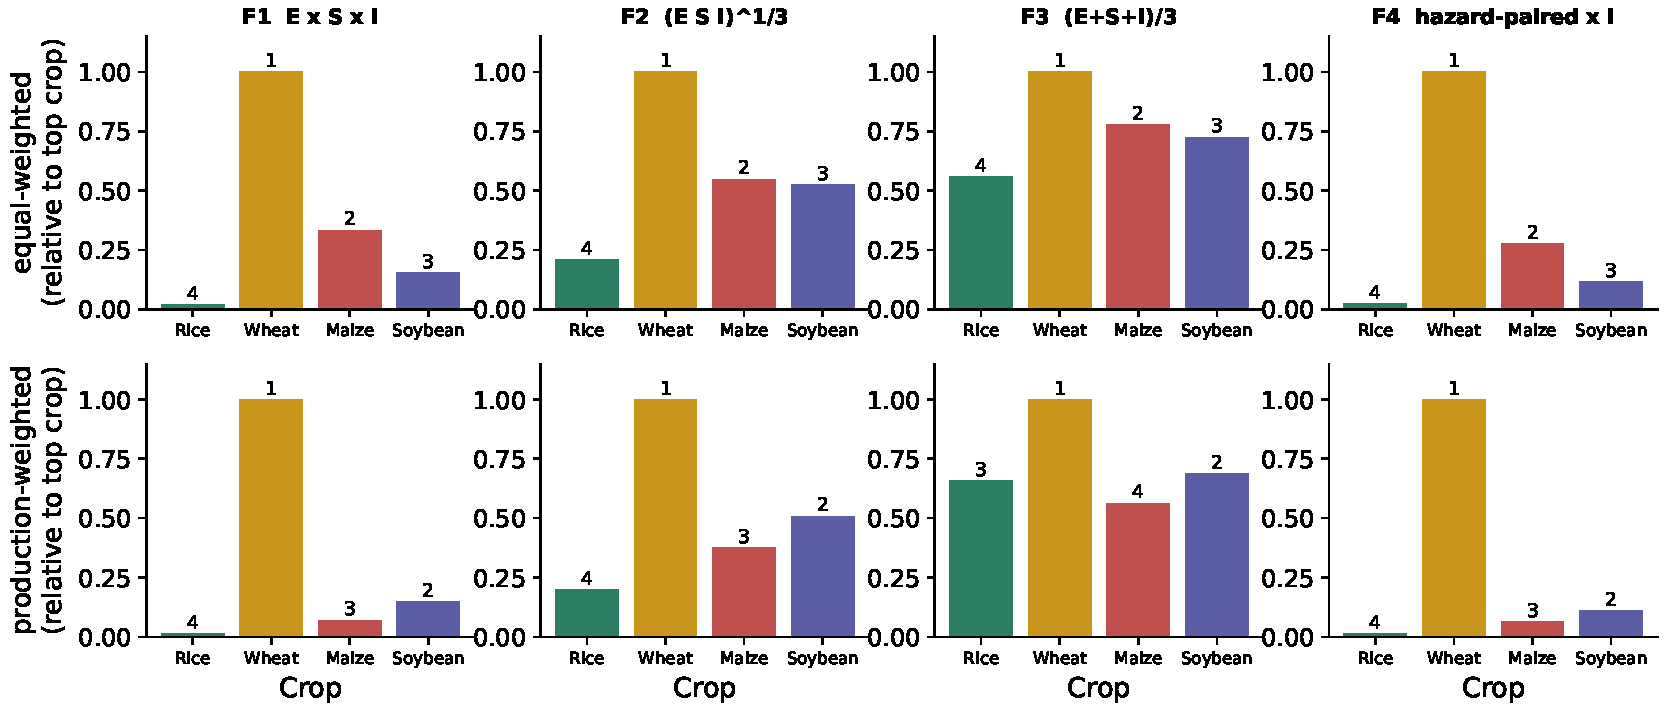
\includegraphics[width=\linewidth]{F08_index_forms.pdf}
\caption{Crop vulnerability across candidate formulas relative to the maximum crop score.}
\end{figure}

% =====================================================================
\section{Supplementary tables}
\begin{table}[H]\centering\tiny
\adjustbox{max width=\linewidth}{\begin{tabular}{llrrrrrrrrrr}
\toprule
 & & \multicolumn{2}{c}{Heat} & \multicolumn{2}{c}{Water} & \multicolumn{2}{c}{Exposure} & \multicolumn{2}{c}{Sensitivity} & & \\
\cmidrule(lr){3-4}\cmidrule(lr){5-6}\cmidrule(lr){7-8}\cmidrule(lr){9-10}
Crop & Country & $L$ (\si{\celsius}) & $\Delta$ (SD) & $L$ (\%) & $\Delta$ (SD) & $E_h$ & $E_w$ & $S_h$ & $S_w$ & $I$ (\%) & $V_{F4}$\\
\midrule
Rice & China (C) & 0.00 & 0.77 & 0.0 & 0.00 & 0.00 & 0.00 & 0.17 & 0.50 & 13.3 & 0.000 \\
 & India (A) & 0.00 & 1.05 & 1.3 & 0.00 & 0.00 & 0.02 & 0.66 & 0.50 & 15.6 & 0.002 \\
 & Bangladesh (A) & 0.00 & 0.87 & 0.1 & 0.12 & 0.00 & 0.00 & 0.17 & 0.50 & 42.1 & 0.000 \\
 & Brazil (A) & 0.00 & 1.08 & 7.6 & 0.06 & 0.00 & 0.14 & 0.17 & 0.50 & 4.7 & 0.004 \\
 & USA (C) & 0.00 & 0.46 & 0.0 & 0.00 & 0.00 & 0.00 & 0.33 & 0.50 & 1.2 & 0.000 \\
 & Nigeria (A) & 0.00 & 0.64 & 7.6 & 0.00 & 0.00 & 0.14 & 0.17 & 0.50 & 5.6 & 0.005 \\
 & Russia (C) & 0.00 & 1.58 & 0.2 & 0.00 & 0.00 & 0.00 & 0.17 & 0.50 & 0.9 & 0.000 \\
\midrule
Wheat & China (C) & 0.01 & 1.34 & 15.0 & 0.01 & 0.02 & 0.27 & 0.37 & 0.44 & 16.0 & 0.024 \\
 & India (C) & 0.58 & 0.90 & 17.8 & 0.02 & 1.00 & 0.33 & 0.43 & 0.44 & 22.2 & 0.151 \\
 & Russia (D) & 0.07 & 0.54 & 31.4 & 0.05 & 0.13 & 0.57 & 0.37 & 0.44 & 31.0 & 0.111 \\
 & USA (D) & 0.08 & 0.24 & 36.9 & 0.01 & 0.13 & 0.68 & 0.37 & 0.44 & 18.2 & 0.075 \\
 & Egypt (B) & 0.08 & 1.46 & 0.1 & 0.00 & 0.14 & 0.00 & 0.37 & 0.44 & 34.4 & 0.021 \\
 & Brazil (C) & 0.01 & 0.96 & 7.3 & 0.25 & 0.02 & 0.13 & 0.37 & 0.44 & 13.3 & 0.010 \\
\midrule
Maize & USA (D) & 0.01 & 0.38 & 16.3 & 0.00 & 0.02 & 0.30 & 0.46 & 0.50 & 2.0 & 0.004 \\
 & China (D) & 0.01 & 0.77 & 8.5 & 0.00 & 0.01 & 0.15 & 0.40 & 0.66 & 1.3 & 0.002 \\
 & Brazil (A) & 0.00 & 0.99 & 13.6 & 0.21 & 0.01 & 0.25 & 0.69 & 0.50 & 6.7 & 0.010 \\
 & India (A) & 0.04 & 0.85 & 3.7 & 0.00 & 0.06 & 0.07 & 0.69 & 0.50 & 1.6 & 0.001 \\
 & S. Africa (B+M) & 0.00 & 0.86 & 36.5 & 0.26 & 0.00 & 0.67 & 0.69 & 0.50 & 22.5 & 0.089 \\
 & Russia (D) & 0.00 & 1.20 & 54.6 & 0.48 & 0.00 & 1.00 & 0.69 & 1.00 & 0.2 & 0.002 \\
\midrule
Soybean & Brazil (A) & 0.00 & 1.08 & 3.8 & 0.13 & 0.00 & 0.07 & 0.76 & 0.42 & 7.3 & 0.002 \\
 & USA (D) & 0.00 & 0.35 & 22.3 & 0.00 & 0.00 & 0.41 & 0.67 & 0.42 & 9.7 & 0.020 \\
 & Argentina (C) & 0.00 & 0.55 & 26.1 & 0.19 & 0.00 & 0.48 & 0.76 & 0.61 & 1.5 & 0.005 \\
 & China (D) & 0.00 & 0.71 & 13.8 & 0.00 & 0.00 & 0.25 & 0.76 & 0.56 & 5.8 & 0.010 \\
 & India (A) & 0.00 & 0.59 & 0.9 & 0.00 & 0.00 & 0.02 & 0.76 & 0.42 & 2.4 & 0.000 \\
 & Russia (D) & 0.00 & 0.63 & 32.5 & 0.09 & 0.00 & 0.60 & 0.76 & 0.42 & 1.1 & 0.003 \\
 & S. Africa (C+M) & 0.00 & 0.83 & 35.4 & 0.33 & 0.00 & 0.65 & 0.76 & 0.42 & 3.8 & 0.012 \\
\bottomrule
\end{tabular}
}
\caption{Index components for each crop--country pair ($L$: level 2001--24; $\Delta$: shift in SDs; $E^{\TT}, E^{\PP}$ scaled 0--1; $S^{\TT}, S^{\PP}$ scaled 0--1; $I$: nutritional share; $V_{F4}$: vulnerability index).}
\end{table}

\begin{table}[H]\centering\tiny
\adjustbox{max width=\linewidth}{\begin{tabular}{lcccc}
\toprule
\textbf{Country} & \textbf{Rice} & \textbf{Wheat} & \textbf{Maize} & \textbf{Soybean} \\
\midrule
USA & $<0.0001$ & 0.0747 & 0.0037 & 0.0197 \\
Brazil & 0.0039 & 0.0103 & 0.0103 & 0.0025 \\
India & 0.0023 & 0.1511 & 0.0015 & 0.0002 \\
China & 0.0001 & 0.0240 & 0.0016 & 0.0097 \\
Russia & $<0.0001$ & 0.1105 & 0.0021 & 0.0032 \\
Argentina & -- & -- & -- & 0.0052 \\
Bangladesh & 0.0002 & -- & -- & -- \\
Egypt & -- & 0.0209 & -- & -- \\
Nigeria & 0.0046 & -- & -- & -- \\
South Africa & -- & -- & 0.0895 & 0.0122 \\
\bottomrule
\end{tabular}
}
\caption{Country-by-crop F4 vulnerability index values ($V_{F4}$).}
\end{table}

\begin{table}[H]\centering\tiny
\adjustbox{max width=\linewidth}{\begin{tabular}{llrrrlrrrlr}
\toprule
 & & \multicolumn{4}{c}{Heat: \% yield per +1\si{\celsius} $T_{eff}$} & \multicolumn{4}{c}{Water: \% yield per +0.1 MR} & \\
\cmidrule(lr){3-6}\cmidrule(lr){7-10}
Crop & Country & lin & quad & FD & used & lin & quad & FD & used & $R^2$\\
\midrule
Rice & China & -1.4 & -0.2 & -0.9 & +0.0 (p) & -0.5 & +0.3 & +0.6 & +0.0 (p) & 0.04\\
 & India & -10.9 & -10.8 & -12.4 & -11.4 (c) & +1.7 & +1.7 & +2.0 & +0.0 (p) & 0.26\\
 & Bangladesh & -5.1 & -4.7 & -4.1 & +0.0 (p) & -0.0 & -0.0 & -0.0 & +0.0 (p) & 0.02\\
 & Brazil & -15.7 & -2.7 & -5.2 & +0.0 (p) & +2.2 & +2.2 & +2.1 & +0.0 (p) & 0.01\\
 & USA & -3.9 & -3.8 & -2.9 & -3.5 (c) & +0.0 & +0.0 & +0.0 & +0.0 (p) & 0.26\\
 & Nigeria & +3.4 & +5.4 & +6.7 & +0.0 (p) & -4.3 & -0.1 & +0.9 & +0.0 (p) & 0.04\\
 & Russia & +6.0 & -5.1 & -3.2 & +0.0 (p) & -4.3 & -18.0 & -13.8 & +0.0 (p) & 0.17\\
\midrule
Wheat & China & -1.8 & -2.0 & +2.0 & -2.7 (p) & +0.3 & +0.2 & -1.7 & +0.0 (p) & 0.02\\
 & India & -4.6 & -4.0 & -4.1 & -4.2 (c) & -2.8 & -1.4 & +0.9 & +0.0 (p) & 0.13\\
 & Russia & +0.2 & -1.2 & +0.5 & -2.7 (p) & +5.5 & +1.9 & +6.8 & +0.0 (p) & 0.19\\
 & USA & -0.1 & -0.1 & -0.3 & -2.7 (p) & +1.8 & +1.8 & +0.7 & +0.0 (p) & 0.13\\
 & Egypt & +0.9 & +0.2 & -1.0 & -2.7 (p) & +2.1 & +2.9 & +0.2 & +0.0 (p) & 0.04\\
 & Brazil & -10.7 & -11.3 & -14.9 & -2.7 (p) & -3.1 & -3.3 & -5.0 & -3.8 (c) & 0.22\\
\midrule
Maize & USA & -5.9 & -5.9 & -7.3 & -6.4 (c) & +0.7 & +0.7 & +0.2 & +0.0 (p) & 0.34\\
 & China & -5.5 & -5.0 & -4.3 & -4.9 (c) & +3.6 & +3.8 & +3.5 & +3.6 (c) & 0.22\\
 & Brazil & -2.6 & -3.2 & -2.5 & -11.7 (p) & +2.1 & +2.1 & +2.0 & +0.0 (p) & 0.05\\
 & India & -11.2 & -10.4 & -10.8 & -11.7 (p) & +0.3 & +0.3 & +0.1 & +0.0 (p) & 0.09\\
 & S. Africa & -25.2 & -27.2 & -31.1 & -27.8 (c) & -3.0 & -4.5 & -1.9 & +0.0 (p) & 0.27\\
 & Russia & +6.7 & +7.6 & +11.3 & -11.7 (p) & +29.1 & +33.5 & +36.5 & +33.0 (c) & 0.50\\
\midrule
Soybean & Brazil & -4.0 & -3.4 & -3.1 & -6.2 (p) & +2.8 & +3.0 & +3.2 & +1.8 (p) & 0.05\\
 & USA & -3.9 & -3.9 & -4.0 & -3.9 (c) & +1.1 & +1.2 & +1.5 & +1.8 (p) & 0.26\\
 & Argentina & +0.4 & -2.3 & -4.9 & -6.2 (p) & +7.0 & +6.7 & +5.3 & +6.3 (c) & 0.54\\
 & China & +4.0 & +1.4 & +4.2 & -6.2 (p) & +5.0 & +5.1 & +5.2 & +5.1 (c) & 0.05\\
 & India & -16.1 & -15.3 & -10.6 & -6.2 (p) & +1.0 & +0.9 & +0.5 & +1.8 (p) & 0.28\\
 & Russia & -17.6 & -10.1 & -8.2 & -6.2 (p) & +14.4 & +18.1 & +16.9 & +1.8 (p) & 0.10\\
 & S. Africa & -17.5 & -11.4 & -15.1 & -6.2 (p) & -5.7 & +1.1 & -2.6 & +1.8 (p) & 0.17\\
\bottomrule
\end{tabular}
}
\caption{Out-of-sample empirical yield regressions over 1971--2000 (lin/quad/FD detrending; used: coefficient entering the data check; $R^2$ of linear model).}
\end{table}

\begin{table}[H]\centering\tiny
\adjustbox{max width=\linewidth}{\begin{tabular}{llrrr}
\toprule
Crop & Country & FBS 1961--2013 & FBS 2010--2023 & MAR pts per 1\% yield\\
\midrule
Rice & China & +0.90$^*$ & -0.31 & -0.000\\
 & India & +0.37$^*$ & +0.54 & +0.025\\
 & Bangladesh & +0.37$^*$ & -0.36 & -0.219\\
 & Brazil & -0.07$^*$ & +0.51 & -0.027\\
 & USA & -0.07 & -0.43 & -0.000\\
 & Nigeria & +0.28 & -0.22 & -0.038\\
 & Russia & +0.21 & -0.83 & -0.000\\
\midrule
Wheat & China & +0.62 & -0.79$^*$ & -0.000\\
 & India & +0.54$^*$ & -0.06 & +0.017\\
 & Russia & -0.04 & +0.09 & -0.000\\
 & USA & -0.19 & -0.04 & -0.000\\
 & Egypt & -0.35$^*$ & -0.02 & -0.000\\
 & Brazil & -0.05 & +0.19 & +0.007\\
\midrule
Maize & USA & -0.13 & -0.01 & -0.000\\
 & China & +0.29 & -0.38 & -0.000\\
 & Brazil & +0.19$^*$ & -0.03 & -0.010\\
 & India & +0.40$^*$ & -1.97 & +0.049\\
 & S. Africa & -0.00 & -0.22 & -0.003\\
 & Russia & +0.31 & -0.82 & -0.000\\
\midrule
Soybean & Brazil & -0.65 & +0.00 & +0.000\\
 & USA & -0.40$^*$ & -0.23$^*$ & -0.000\\
 & Argentina & +1.59$^*$ & +0.03 & +0.004\\
 & China & +0.10 & +0.37 & +0.000\\
 & India & -1.84 & -0.09 & +0.009\\
 & Russia & +1.56$^*$ & +3.04$^*$ & +0.000\\
 & S. Africa & +1.83$^*$ & +0.08 & -0.003\\
\bottomrule
\end{tabular}
}
\caption{Yield pass-through to food supply and MAR (FBS 1961--2013 and 2010--2023).}
\end{table}

\begin{table}[H]\centering\tiny
\adjustbox{max width=\linewidth}{\begin{tabular}{llrrrrrrr}
\toprule
 & & & \multicolumn{2}{c}{Climate-driven $\Delta Y$ (\%)} & \multicolumn{4}{c}{Standard $-10$\% yield shock (S3)}\\
\cmidrule(lr){4-5}\cmidrule(lr){6-9}
Crop & Country & SSR & S1 shift & S2 1-in-10 & $\Delta$kcal\% & $\Delta$Zn\% & $\Delta$Fe\% & $\Delta$MAR pts (no trade / trade)\\
\midrule
Rice & China & 0.95 & +0.0 & +0.0 & -2.36 & -1.51 & -0.82 & +0.00 / +0.00\\
 & India & 1.19 & -4.8 & -3.3 & -2.47 & -2.09 & -1.15 & -0.20 / -0.00\\
 & Bangladesh & 1.02 & +0.0 & +0.0 & -6.29 & -5.45 & -3.62 & -0.50 / -0.51\\
 & Brazil & 1.04 & +0.0 & +0.0 & -0.78 & -0.59 & -0.40 & -0.08 / +0.00\\
 & USA & 1.43 & -1.4 & -2.7 & -0.21 & -0.15 & -0.11 & +0.00 / +0.00\\
 & Nigeria & 1.00 & +0.0 & +0.0 & -0.83 & -0.76 & -0.37 & -0.07 / -0.07\\
 & Russia & 0.79 & +0.0 & +0.0 & -0.12 & -0.09 & -0.06 & +0.00 / +0.00\\
\midrule
Wheat & China & 0.90 & -3.7 & -4.0 & -1.62 & -1.92 & -1.72 & +0.00 / +0.00\\
 & India & 1.01 & -3.2 & -4.1 & -2.11 & -3.26 & -2.95 & -0.52 / -0.28\\
 & Russia & 1.78 & -3.1 & -4.8 & -2.91 & -4.56 & -4.90 & +0.00 / +0.00\\
 & USA & 1.25 & -1.1 & -4.8 & -1.54 & -2.72 & -3.09 & +0.00 / +0.00\\
 & Egypt & 0.56 & -3.6 & -3.3 & -1.90 & -2.70 & -2.57 & +0.00 / +0.00\\
 & Brazil & 0.69 & +1.1 & -16.8 & -0.75 & -1.41 & -1.57 & -0.31 / +0.00\\
\midrule
Maize & USA & 1.20 & -2.8 & -4.6 & -0.21 & -0.29 & -0.33 & +0.00 / +0.00\\
 & China & 0.92 & -2.8 & -4.4 & -0.15 & -0.16 & -0.14 & +0.00 / +0.00\\
 & Brazil & 1.55 & -7.0 & -6.1 & -0.72 & -0.92 & -1.05 & -0.20 / +0.00\\
 & India & 1.15 & -4.6 & -2.7 & -0.18 & -0.23 & -0.21 & -0.04 / -0.00\\
 & S. Africa & 1.36 & -26.8 & -23.8 & -2.17 & -2.95 & -3.23 & -0.53 / -0.00\\
 & Russia & 1.28 & -38.1 & -31.4 & -0.02 & -0.03 & -0.03 & +0.00 / +0.00\\
\midrule
Soybean & Brazil & 2.52 & -4.3 & -4.3 & -0.98 & -0.00 & -0.01 & -0.00 / +0.00\\
 & USA & 1.65 & -0.8 & -3.9 & -1.43 & -0.00 & -0.01 & +0.00 / +0.00\\
 & Argentina & 0.97 & -4.6 & -16.9 & -0.20 & -0.00 & -0.00 & +0.00 / +0.00\\
 & China & 0.27 & -2.6 & -7.6 & -0.10 & -0.08 & -0.18 & +0.00 / +0.00\\
 & India & 0.82 & +0.8 & -8.9 & -0.17 & -0.01 & -0.03 & -0.01 / -0.01\\
 & Russia & 1.02 & -4.4 & -4.9 & -0.13 & -0.00 & -0.01 & +0.00 / +0.00\\
 & S. Africa & 1.13 & -7.1 & -6.6 & -0.43 & -0.03 & -0.09 & -0.01 / -0.00\\
\bottomrule
\end{tabular}
}
\caption{Nutritional impact under yield shock scenarios (S1 observed shift, S2 1-in-10 shock, S3 $-10$\% standard shock).}
\end{table}

% =====================================================================
\section{Supplementary figures}
\begin{figure}[H]\centering
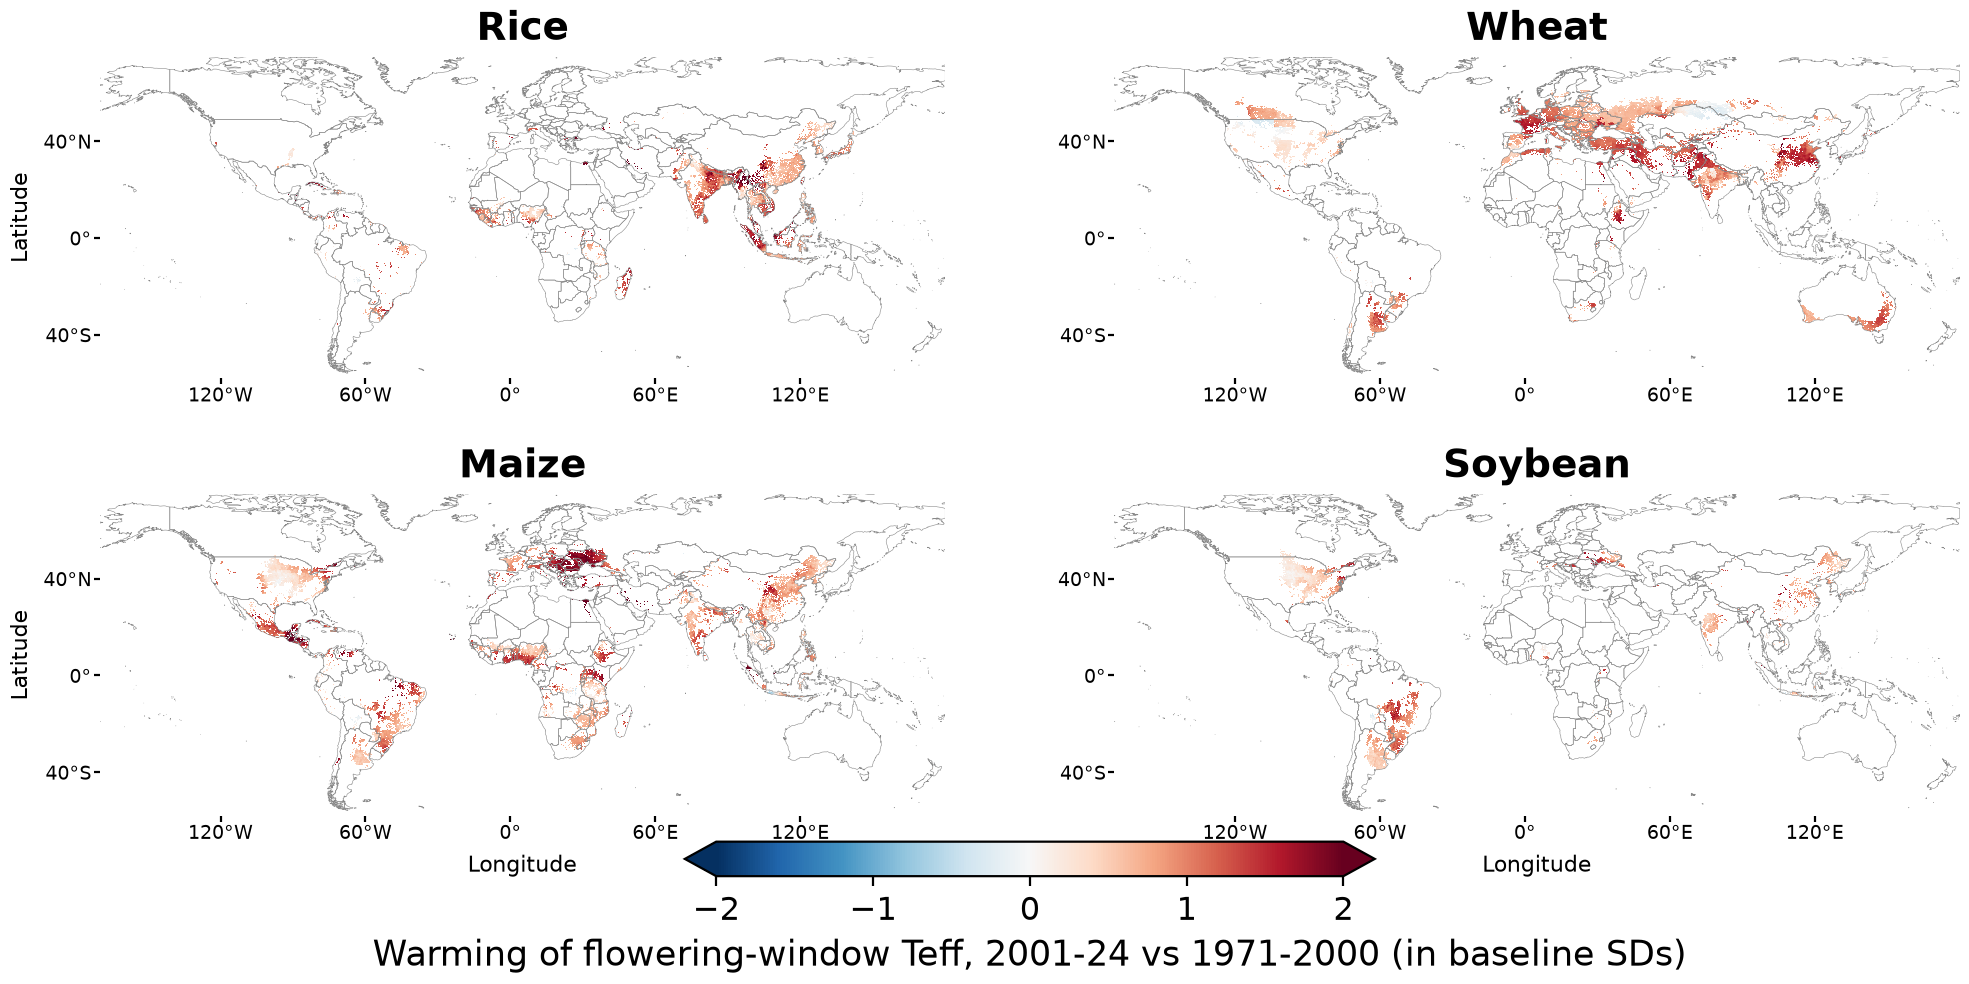
\includegraphics[width=\linewidth]{F02a_heat_shift_map.png}
\caption{Warming of the flowering season (2001--2024 vs 1971--2000 baseline SDs).}
\end{figure}

\begin{figure}[H]\centering
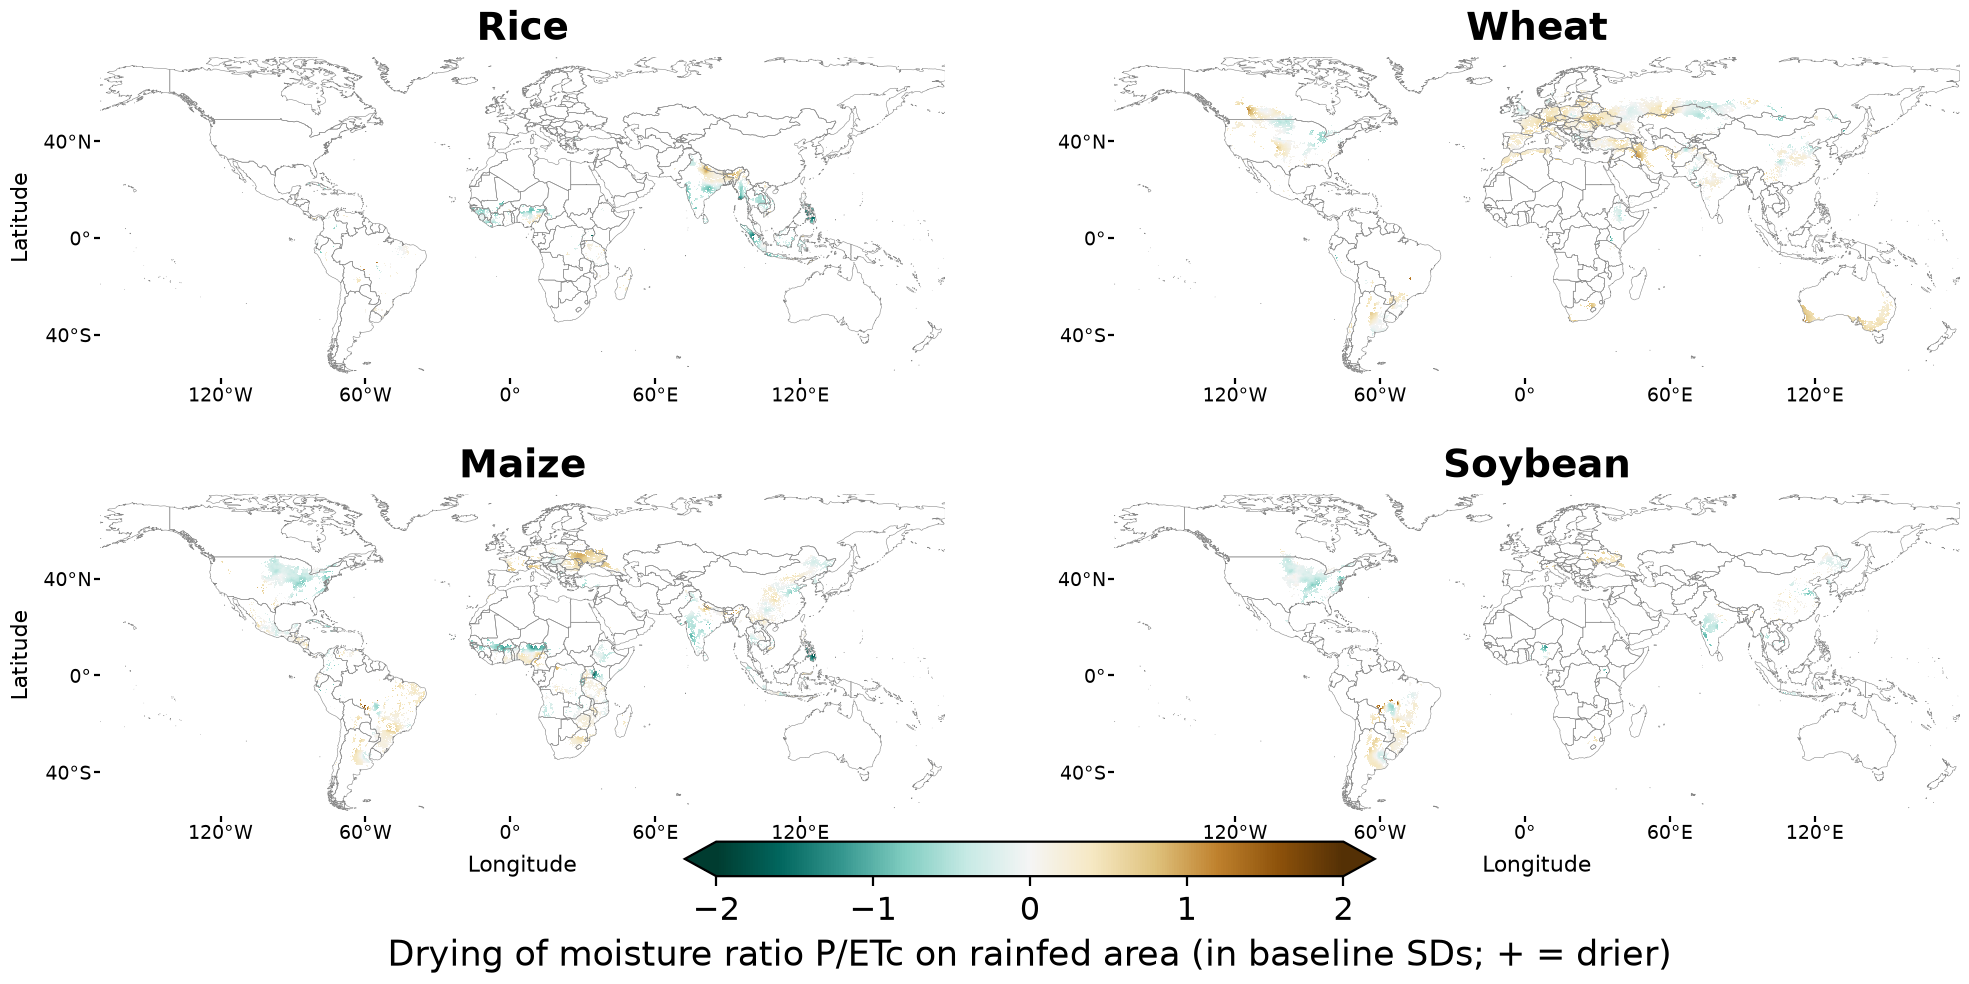
\includegraphics[width=\linewidth]{F02b_water_shift_map.png}
\caption{Drying of the rainfed growing season (shift in moisture ratio $P/ET_c$ in baseline SDs).}
\end{figure}

\begin{figure}[H]\centering
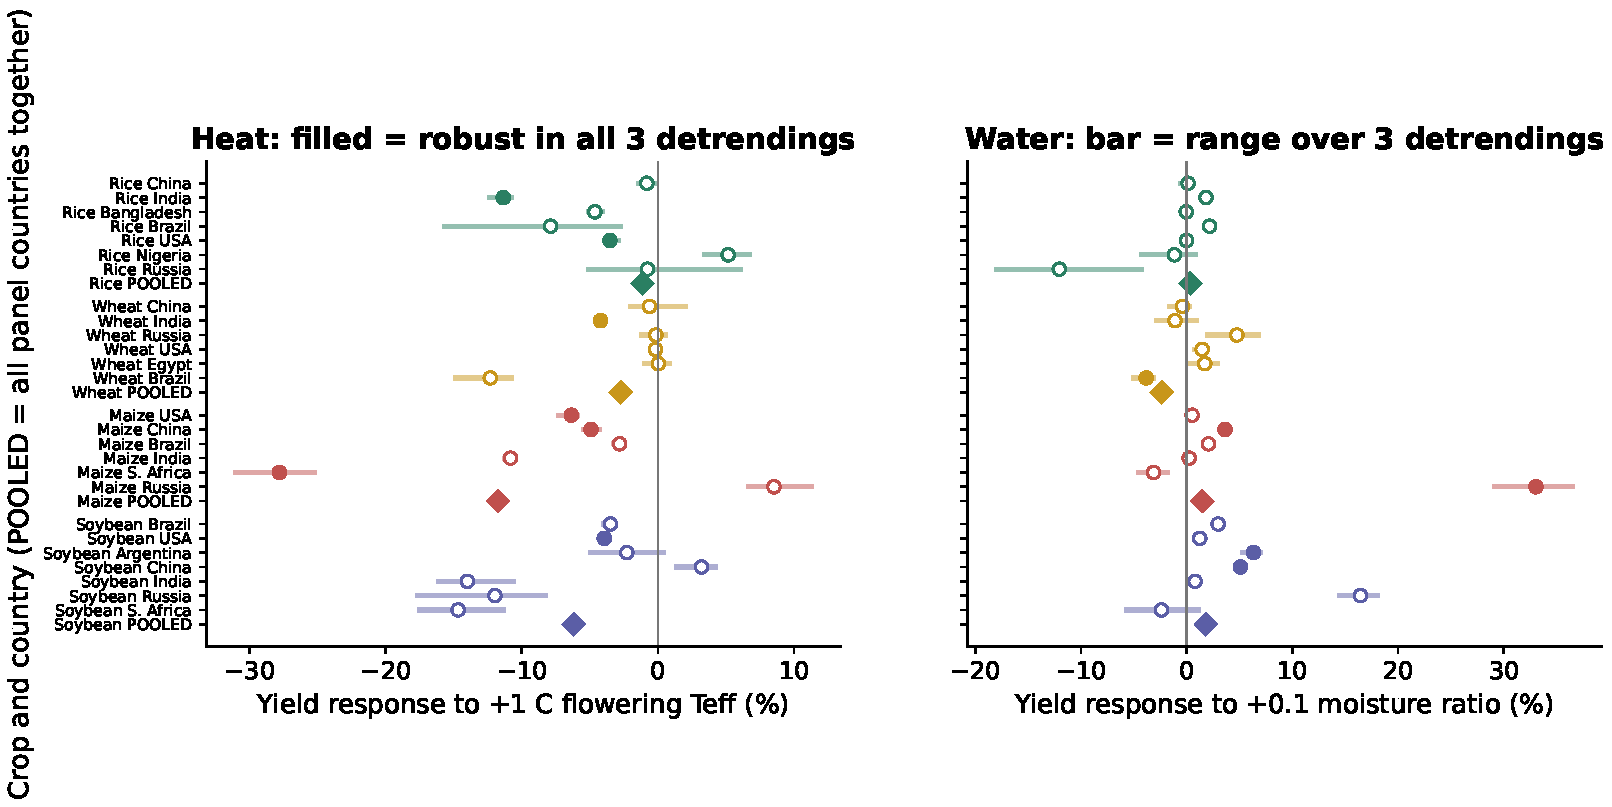
\includegraphics[width=\linewidth]{F05_sensitivity_coefficients.pdf}
\caption{Observed yield sensitivity coefficients by crop and country.}
\end{figure}

\begin{figure}[H]\centering
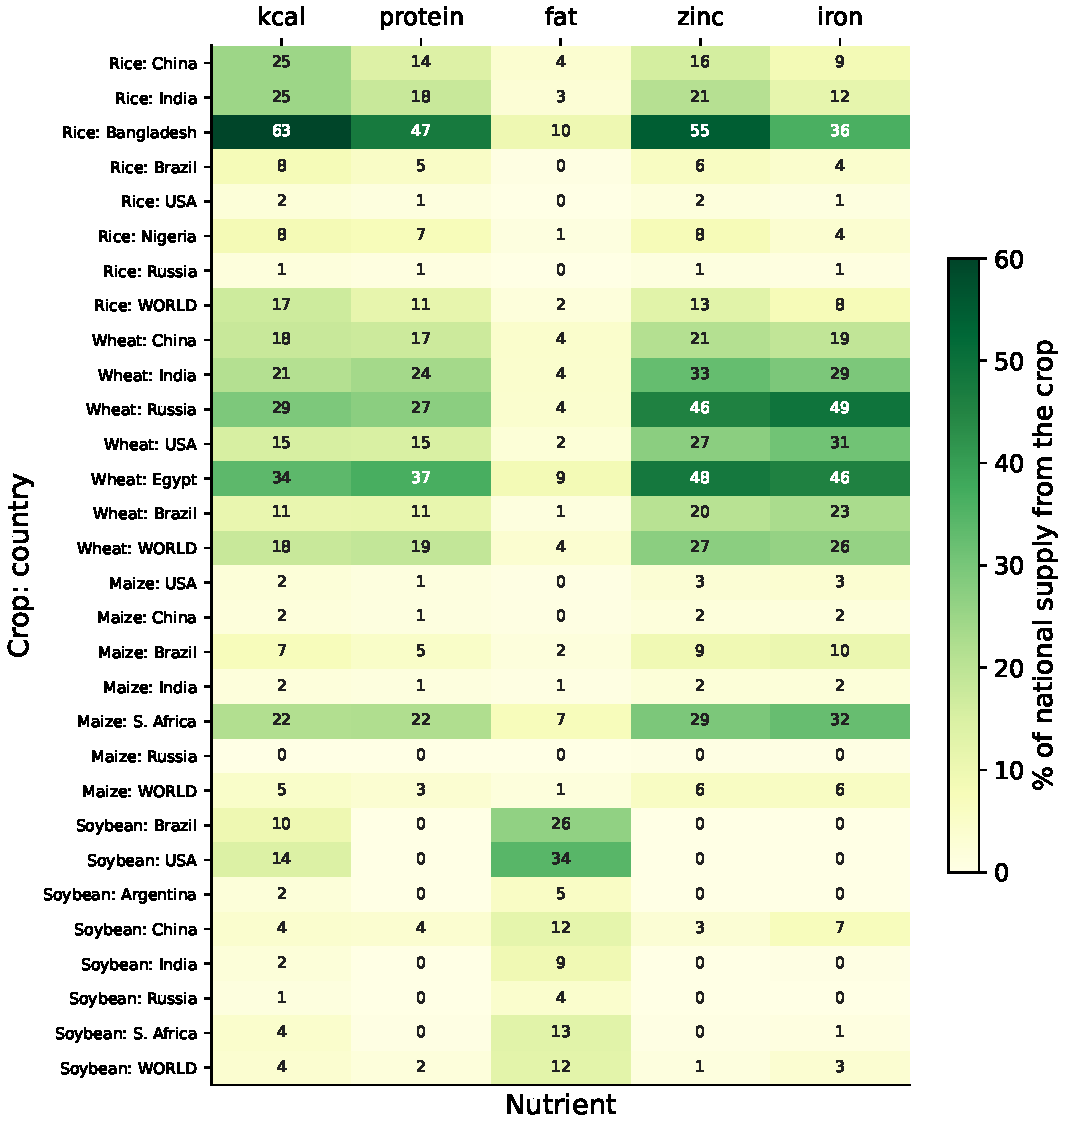
\includegraphics[width=0.7\linewidth]{F06_importance_heatmap.pdf}
\caption{Nutritional supply share heatmap across all 5 nutrients by crop and country.}
\end{figure}

\begin{figure}[H]\centering
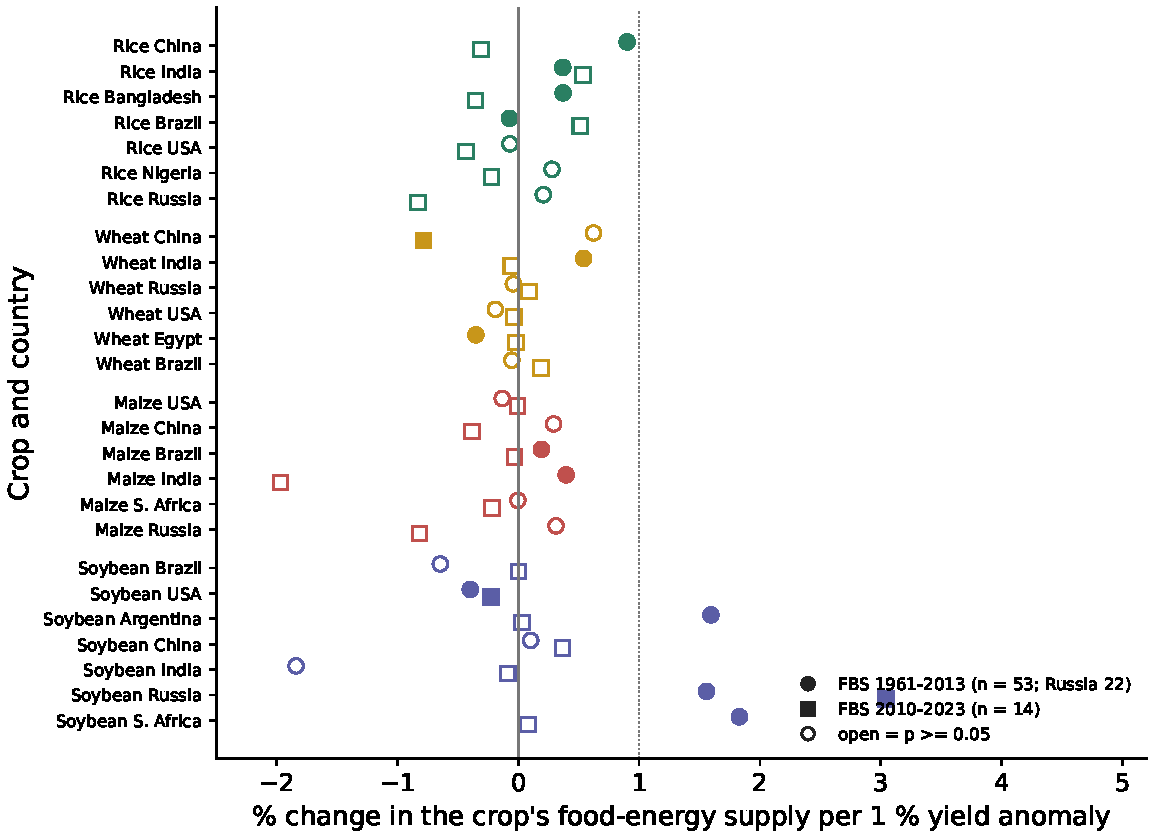
\includegraphics[width=0.85\linewidth]{F13_yield_supply_passthrough.pdf}
\caption{Yield-to-supply pass-through regression coefficients across countries.}
\end{figure}

\begin{figure}[H]\centering
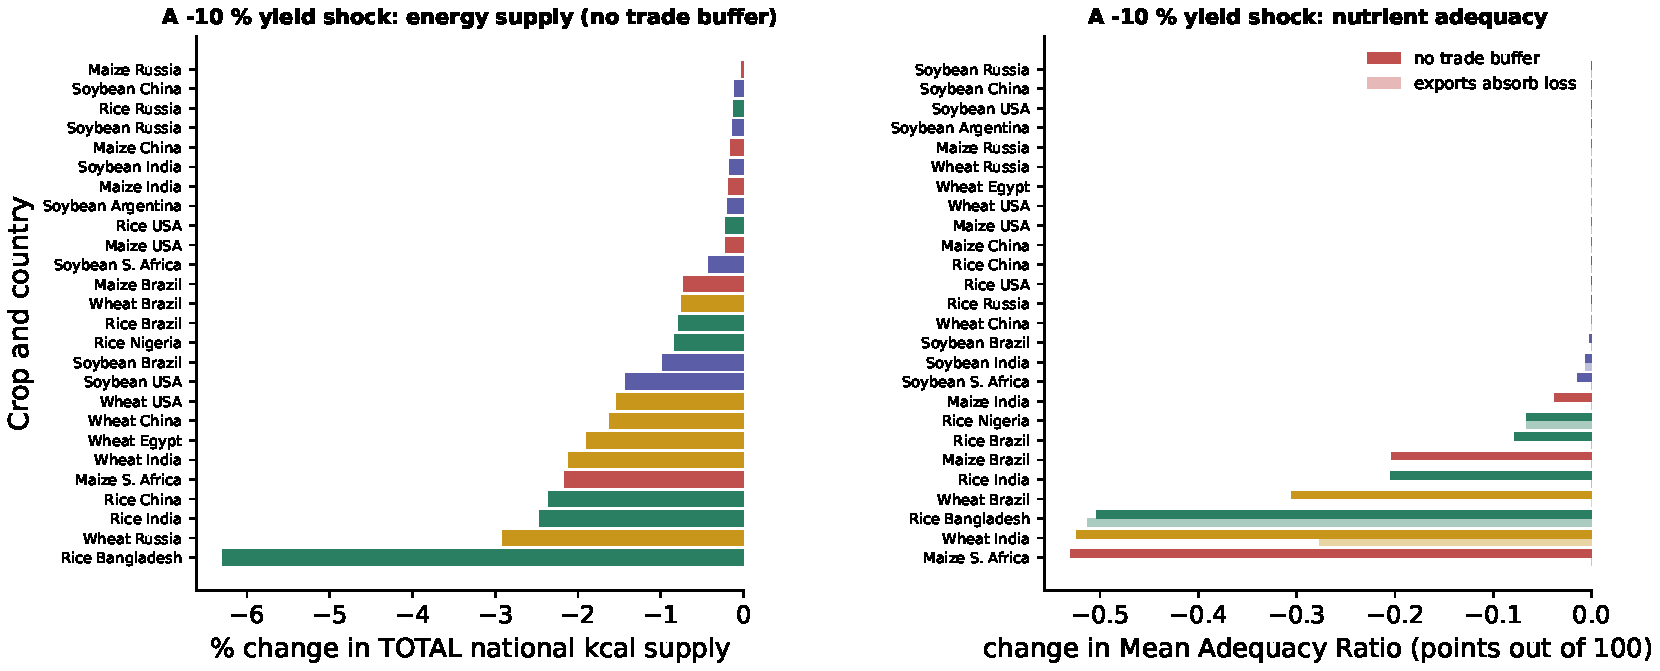
\includegraphics[width=\linewidth]{F14_scenario_shock.pdf}
\caption{Impact of a $-10$\% yield shock on calories and Mean Adequacy Ratio (MAR).}
\end{figure}

% =====================================================================
\section{Robustness and validation}\label{sec:robust}
\subsection{Robustness}
A series of 10 one-at-a-time modifications was evaluated (min--max normalization, level vs shift exposure, literature vs empirical sensitivity modes, rice $K_y$ proxies, and calorie-only vs micronutrient-only importance). Across all \robN\ tests, \textbf{wheat is ranked \#1 in \robWheatTopAll\ cases}. Monte Carlo simulation (2,000 Dirichlet draws) places wheat first in \mcFourWheatFirst\% of iterations under F4.

\begin{table}[H]\centering\scriptsize
\adjustbox{max width=\linewidth}{\begin{tabular}{lll}
\toprule
Test (one choice changed) & F4 hazard-paired order & F1 multiplicative order\\
\midrule
main (x/max, exposure = stress level, lit+emp S) & wheat $>$ maize $>$ soybean $>$ rice & wheat $>$ maize $>$ soybean $>$ rice \\
min-max normalisation & wheat $>$ maize $>$ soybean $>$ rice & wheat $>$ maize $>$ soybean $>$ rice \\
exposure = level + change (average) & wheat $>$ maize $>$ rice $>$ soybean & wheat $>$ maize $>$ rice $>$ soybean \\
exposure = change only & wheat $>$ maize $>$ rice $>$ soybean & wheat $>$ maize $>$ rice $>$ soybean \\
sensitivity = literature only & wheat $>$ maize $>$ soybean $>$ rice & wheat $>$ maize $>$ soybean $>$ rice \\
sensitivity = empirical only & wheat $>$ soybean $>$ maize $>$ rice & wheat $>$ maize $>$ soybean $>$ rice \\
rice Ky = 1.0 & wheat $>$ maize $>$ soybean $>$ rice & wheat $>$ maize $>$ soybean $>$ rice \\
rice Ky = 1.5 & wheat $>$ maize $>$ soybean $>$ rice & wheat $>$ maize $>$ soybean $>$ rice \\
importance = kcal share only & wheat $>$ maize $>$ soybean $>$ rice & wheat $>$ maize $>$ soybean $>$ rice \\
importance = Zn+Fe+protein only & wheat $>$ maize $>$ rice $>$ soybean & wheat $>$ maize $>$ soybean $>$ rice \\
\bottomrule
\end{tabular}
}
\caption{Crop ranking under each one-at-a-time robustness test.}\label{tab:robust}
\end{table}

\begin{figure}[H]\centering
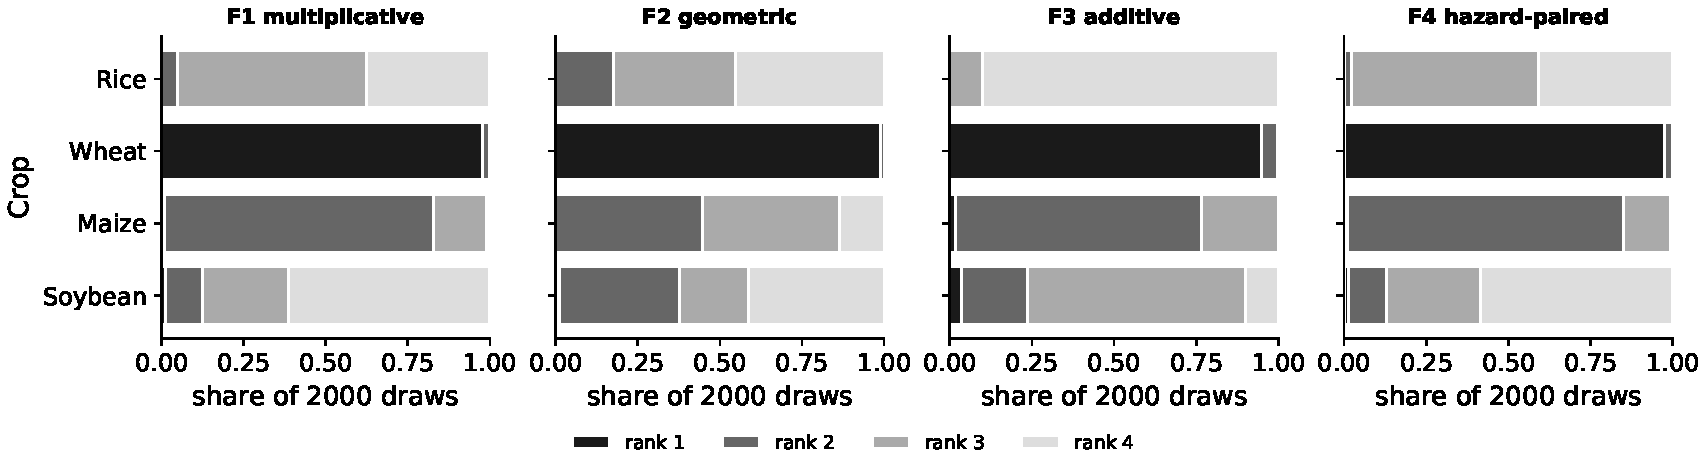
\includegraphics[width=0.85\linewidth]{F10_montecarlo_ranks.pdf}
\caption{Rank distribution from 2,000 Monte Carlo draws of component sub-weights.}
\end{figure}

\subsection{Validation Benchmarks}
\begin{itemize}
\item \textbf{Zhao et al. (2017):} Comparison against published multi-model warming yield loss shows rank agreement $\rho=\rhoZhaoFour$.
\item \textbf{Myers et al. (2014):} Elevated CO$_2$ declines in zinc, iron, and protein disproportionately impact wheat and rice, confirming their vulnerability in our nutritional weighting.
\item \textbf{Ray et al. (2015):} Climate-explained yield variability checks confirm that rice exhibits the lowest climate variability share among the four crops.
\end{itemize}

\begin{figure}[H]\centering
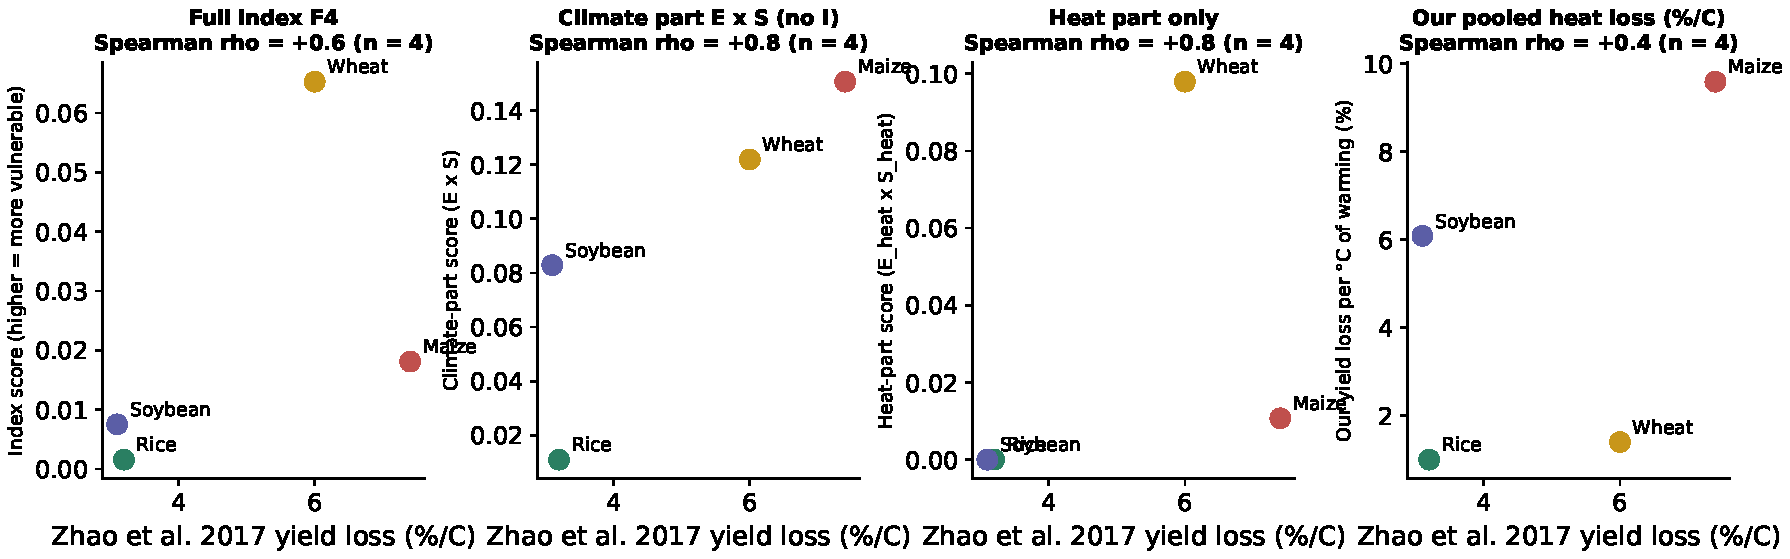
\includegraphics[width=\linewidth]{F11_zhao_validation.pdf}
\caption{Crop vulnerability index scores compared with Zhao et al. (2017) global yield loss per \si{\celsius}.}
\end{figure}

\bibliography{refs}

\end{document}


